\documentclass{article}


\usepackage{arxiv}

\usepackage[utf8]{inputenc} % allow utf-8 input
\usepackage[T1]{fontenc}    % use 8-bit T1 fonts
\usepackage{hyperref}       % hyperlinks
\usepackage{url}            % simple URL typesetting
\usepackage{booktabs}       % professional-quality tables
\usepackage{amsfonts}       % blackboard math symbols
\usepackage{nicefrac}       % compact symbols for 1/2, etc.
\usepackage{microtype}      % microtypography
\usepackage{lipsum}
\usepackage{graphicx}
\usepackage{tabularx}% <-- added
\usepackage[export]{adjustbox}% <-- added
\graphicspath{ {./images/} }

\title{Multi-label multi-class text classification: DPCNN stacked with XLNet, BERT and RoBERTa}


\author{
  Marcelo Blinder \\
  \texttt{mblinder@berkeley.edu} \\
   \And
 Carlos Sancini \\
  \texttt{carlos.sancini@berkeley.edu} \\
}

\begin{document}
\maketitle

\begin{abstract}
In this paper we show that a deep learning ensemble composed of a DPCNN stacked on top of XLNet, BERT or RoBERTa, leads to a classifier with higher performance compared to that of XLNet, BERT or RoBERTa alone. This result was achieved in New York Times Annotated Corpus and encompassed the re-implementation of several classes from the Transformers package with the objectives of training the DPCNN while fine-tuning XLNet, BERT and RoBERTa, as well as the replacement of the loss computation, since the multi-label multi-class classification task requires the calculation of the cross-entropy directly with the individual logits of each class instead of a SoftMax.
\end{abstract}

\section{INTRODUCTION}

A multi-class multi-label classification problem is a supervised learning problem in which an observation can be associated simultaneously with multiple labels. An example of this type of task is The New York Times Annotated Corpus that contains news and corresponding labels that classifies the type of content, e.g. Economy and Technology, if the content of the article contains information related to both subjects.  Due to this nature, the multi-label text classification task is often considered to be more challenging compared to the binary or multi-class text classification problems.

This is an important task with applications in medicine, such as assigning diagnosis codes to a medical report, the financial industry, and such as assigning stock codes to news and deriving its positive, neutral or negative impact. We chose the New York Times corpus since it is as challenging as the other mentioned tasks; however, it does not require specific domain knowledge.

Our approach to address this classification task was to use deep learning ensemble methods based on the Deep Pyramid Convolutional Neural Network (DPCNN)\cite{dpcnn_ref} architecture. In the first ensemble, we stacked together DPCNN and XLNet\cite{xlnet_ref}, in the second, DPCNN and BERT\cite{bert_ref} and in a third DPCNN and RoBERTa\cite{roberta_ref}. By the time that DPCNN was proposed, transfer learning was advancing, and its architecture considered the use of embeddings with the neural network; however, we leverage not only the embeddings generated by XLNet, BERT or RoBERTa, but also the fine tuning capability of these methods. In simple terms, we trained the DPCNN while fine tuning XLNet, BERT and RoBERTa in conjunction. 

To compare the results of these ensemble methods, we established our own baseline by fine tuning XLNet, BERT and RoBERTa individually, without the DPCNN. We took this path since we couldn’t access the results and details of official sources that attempted to solve this classification problem. Therefore, we will present in this paper the performance of 3 ensemble methods and 3 baseline comparison methods, for a total of 6 models.

In section \ref{background_section} we make a brief theoretical background introduction. Section \ref{models_section} contains the model architecture details when using XLNet, BERT, RoBERTa and DPCNN stacked together.  It also contains a description of the python packages used and the python packages modified to create the ensembles. In section \ref{dataset_section}  we present in detail the dataset and the choices we made for tokenization. In section \ref{metrics_section} we conduct a discussion about the metrics used for the multilabel multiclass task. In section \ref{result_section} we present and analyze the results of the 6 models. In section \ref{conclusion_section} we state the conclusion of our work and describe further strategies that we think would further improve performance of the New York Times classification task.

\section{DATASET} \label{dataset_section}

The corpus is maintained by The New York Times Research \& Development team and is  drawn from the historical archive of The New York Times. It includes metadata provided by The New York Times Newsroom, The New York Times Indexing Service and the online production staff at NYTimes.com. This corpus contains nearly every article published in The New York Times between January 01, 1987 and June 19, 2007\cite{nyt_corpus_ref} and advertisements. For this project only news article were used.

The dataset contains 788,503 observations and each observation can be associated with up to 12 labels. Figure \ref{fig:labels_frequency_and_num_classes} shows the number of labels vs number of observations in the dataset and the distribution of labels in the corpus is uneven and some classes are very skewed, such as Education that is present in 0.88\% of observations whereas Business is present in 27.54\%. In the results section it is possible to see that the individual accuracy for skewed classes are worse, as expected.

One example of a text with multiple labels is shown in Example 1, see \ref{appendix_example_1}. The headline and the article itself are both concatenated in the dataset. We kept the text this way when we trained our models since we believe that the headline and the first paragraph would contain useful information for the classification task. We also noticed that not all texts have a headline, as Example 2 (see \ref{appendix_example_2}) which is a short text article with just one label and is entirely shown below. The example 1 is a long text and it is shown only the headline and the first two paragraphs. The full text can be found in the appendix.

The number of tokens in each news article also presented an accuracy offender, since most of the texts in the corpus were long. Figure \ref{fig:density_tokens} shows a density plot of tokens for the texts in the dataset. We had to limit the number of tokens for each observation to only 128 for BERT and XLNet and 100 for RoBERTa since we faced out-of-memory issues during training, especially with XLNet. We are aware that we would achieve higher accuracy if we had used 1024 or 2048, but that would have required a more sophisticated training infrastructure. The tokenization process itself was slow and took a couple of hours to complete due to the large size of the texts in the corpus.

\begin{figure}
    \centering
    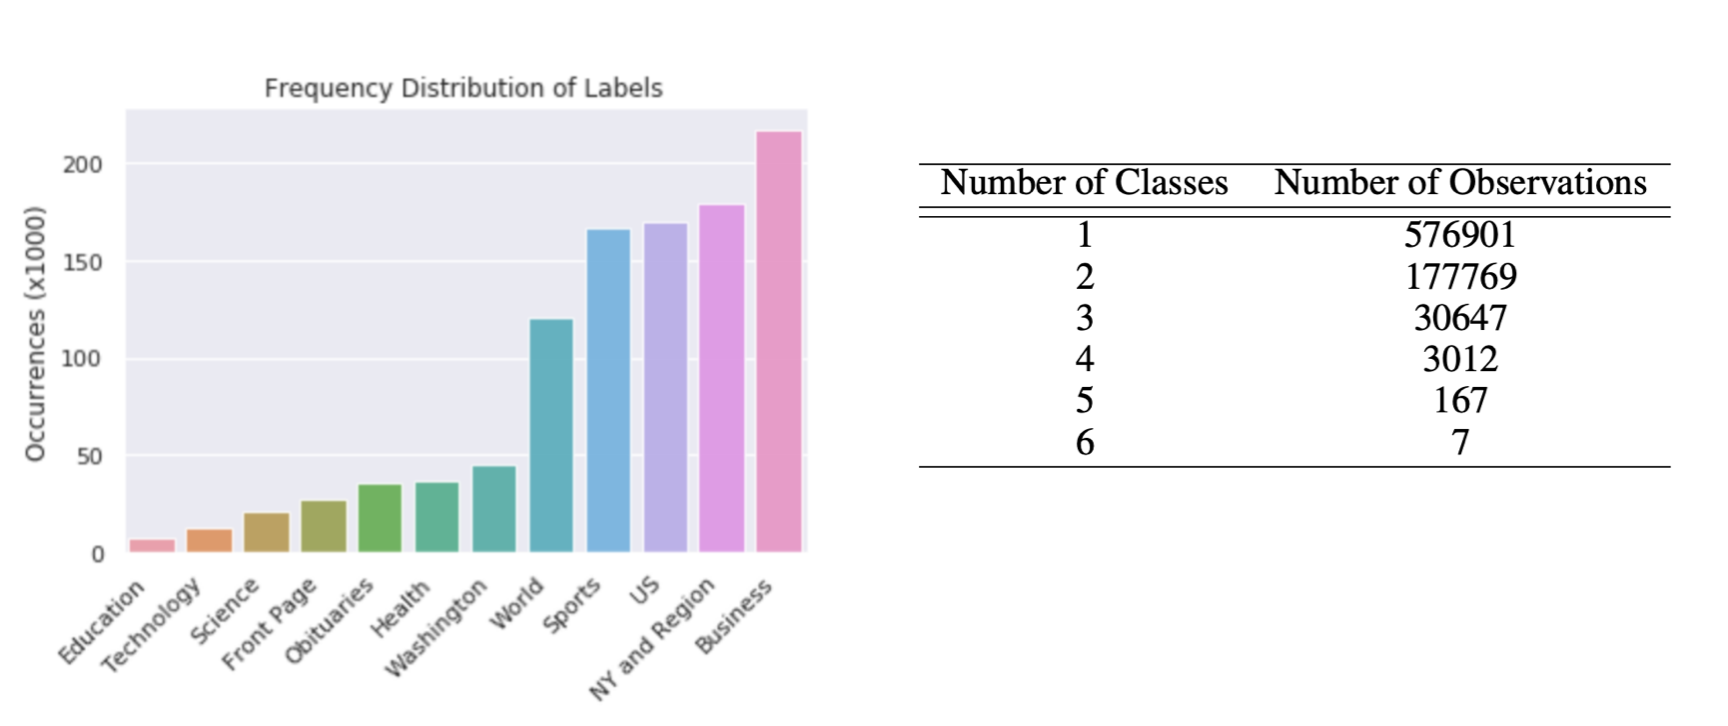
\includegraphics[scale=0.4]{images/labels_and_num_classes.png}
    \caption{Frequency of each label in the dataset and number of observations per class}
    \label{fig:labels_frequency_and_num_classes}
\end{figure}

Data preparation of the corpus was straightforward since all the files are well organized and documented by The NYT. It took a simple python scripts to iterate over the files of each year and extract the information we needed, the news articles themselves and the corresponding classes, which we transformed to a one-hot encoding format. Next, tokenization of the corpus was achieved with both SentencePiece\cite{sentencepiece_ref}, when training XLNet alone and XLNet with DPCNN, and BPE\cite{machine_translation_ref}, when training BERT alone and BERT with DPCNN. This choice only reflects the original implementation of either XLNet or BERT/RoBERTa.

After tokenization, we limited the number of tokens to 128 for BERT and XLNet and 100 for RoBERTa and padded with zeros the texts that were smaller than 128 or 100 tokens. Before that we included the special tokens (<SEP> and <CLS>) for BERT and XLNet and (<s> and </s>) for RoBERTa. From there, we created vectors with the input ids, which contained the tokens ids from the XLNet or BERT vocabulary, the input masks, which contained a series of ones for real tokens and zeros for padding tokens, and the segment ids, which contained only zeros since the task at hand involved only one sentence (as opposed to sentence-to-sentence tasks that would have required zeros to mark the tokens of the first sentence and ones for the second).

\section{BACKGROUND} \label{background_section}

This theoretical background contains adapted key extractions from original DPCNN, XLNet, BERT and RoBERTa papers. The objective of this section is to highlight important concepts that made part of our work and to make easy to understand the proposed ensemble in section \ref{models_section}.

\subsection{CNN and RNN}

A CNN is a feedforward network with convolution layers interleaved with pooling layers. Basically, a convolution layer converts to a vector every small patch of data (either the original data such as text or image or the output of the previous layer) at every location (e.g., 3-word windows around every word), which can be processed in parallel.

By contrast, an RNN has connections that form a cycle. In its typical application to text, a recurrent unit takes words one by one as well as its own output on the previous word, which is parallel-processing unfriendly. The drawback of RNN is that it is does not perform well when long range dependencies are needed for the task. 

While both CNNs and RNNs can take advantage of word order, the simple nature and parallel-processing friendliness of CNNs make them attractive particularly when large training data causes computational challenges.

\subsection{DPCNN}

The DPCNN attempts to overcome the problems of an RNN. Its architecture is in essence a CNN, but its implementation alternates a convolution block and a downsampling layer over and over, leading to a deep network in which internal data size (as well as per-layer computation) shrinks in a pyramid shape. The advantage of a DPCNN is that  the ‘pyramid’ enables efficient discovery of long-range associations in the text (and so more global information than an RNN), as the network is deepened, while still keeping the benefits of parallel computation of a CNN.

The schematic shown in Figure \ref{fig:bert_dpcnn_architecture} illustrates the DPCNN architecture. The first layer performs text region embedding. Later we show that we replaced this first by either XLNet, BERT or RoBERTa. It is then followed by stacking of convolution blocks (two convolution layers and a shortcut) interleaved with pooling layers with stride 2 for downsampling. The final pooling layer aggregates internal data for each document into one vector (max pooling for all pooling layers). Later in section \ref{models_section}, we show how we aggregated to the last DPCNN pooling layer a final classification layer, in which logits were used to calculate the loss (further details about the loss function of the ensemble are given in section \ref{metrics_section}). 

\subsection{Pre-training and fine tuning}

There are two existing strategies for applying pre-trained language representations to downstream tasks: feature-based and fine-tuning. The feature-based approach, such as ELMo\cite{deepcontextualized_word_ref}, uses task-specific architectures that include the pre-trained representations as additional features. The fine-tuning approach, such as BERT and XLNet, introduces minimal
task-specific parameters and is trained on the downstream tasks by simply fine-tuning all pretrained parameters. The two approaches share the same objective function during pre-training, where they use unidirectional language models to learn general language representations. In this paper we applied the fine-tuning strategy of XLNet and BERT/RoBERTa.

These pre-trained language representations are unsupervised representation learning that have been highly successful in the domain of natural language processing. Typically, these methods first pretrain neural networks on large-scale unlabeled text corpora, and then finetune the models or representations on downstream tasks. While BERT and RoBERTa applies the autoencoding (AE), ELMo applies the autoregressive (AR) concept, XLNet is a method that attempts to overcome the limitations of AR and AE, while keeping their benefits, in a concept called generalized autoregression.

\subsection{BERT}

BERT aims to reconstruct the original data from corrupted input. Given the input token sequence, a certain portion of tokens are replaced by a special symbol [MASK], and the model is trained to recover the original tokens from the corrupted version. BERT is designed to pre-train deep bidirectional representations from unlabeled text by jointly conditioning on both left and right context in all layers. As a result, the pre-trained BERT model can be finetuned with just one additional output layer to create a model for a specific task, such as the classification task of the NYT corpus, without substantial task specific architecture modifications. Later in section \ref{models_section}, we show that for this last output layer we actually used a full DPCNN.

The fine-tuning based approach proposed in BERT (Bidirectional Encoder Representations from Transformers) alleviates the problems associated with previous unidirectionality constraint of earlier models, such as OpenAI GPT\cite{improving_language_understanding_ref}, by using a “masked language model” (MLM) pre-training objective that enables the learning of a representation that fuses the left and the right contexts simultaneously. The result is a pre-trained deep bidirectional Transformer.

\subsection{XLNet}

A drawback of BERT is that it is not able to model the joint probability using the product rule as in AR language modeling. In other words, BERT assumes the predicted tokens are independent of each other given the unmasked tokens, which is oversimplified as high-order, long-range dependency is prevalent in natural language.

Instead of using a fixed forward or backward factorization order as in conventional AR models, XLNet maximizes the expected log likelihood of a sequence, i.e. all possible permutations of the factorization order. With the  permutation operation, the context for each position can consist of tokens from both left and right. In expectation, each position learns to utilize contextual information from all positions, capturing bidirectional context. In this way, XLNet does not rely on “data corruption” and does not suffer from the pretrain-finetune discrepancy that BERT is subject to. Meanwhile, the autoregressive objective also provides a natural way to use the product rule for factorizing the joint probability of the predicted tokens . The elimination of the independence granted XLNet a considerable performance improvement over BERT.

XLNet also integrated the segment recurrence mechanism and relative encoding scheme of Transformer-XL  into pretraining, which also improved the performance especially for tasks involving a longer text sequence. In section 4 we show that this is the case of the NYT corpus, which contain long new articles.

\subsection{RoBERTa}

RoBERTa claims that BERT was undertrained and that the hyperparameter tuning can be improved. RoBERTa improves on BERT by training the model on longer, bigger batches; removing the next sentence prediction objective; training on longer sentences; and dynamically changing the masking pattern on the training data. The model was also trained on larger datasets. 

\section{MODELS} \label{models_section}

Our approach to improve the NYT classification task was to stack a DPCNN on top of BERT, XLNet and RoBERTa. In other words, the last classification layers of BERT, XLNet and RoBERTa were replaced by a more complex DPCNN classification stage. In this way, we aimed to leverage the pre-learned embeddings/language model in a more robust fine-tuning setting. Figure \ref{fig:bert_dpcnn_architecture} illustrates how BERT was connected to the DPCNN. For BERT, the last layer of (Number of words, 768) was used connected to the DPCNN with 250 channels and 2 convolutions followed by downsampling. Similarly, the same type of architecture was used for XLNet and RoBERTa. During hyperparameter fine-tuning we also find out that two dropout layers, one before the connection with DPCNN and another before loss computation, led to better results. 

\clearpage
\begin{figure}
    \centering
    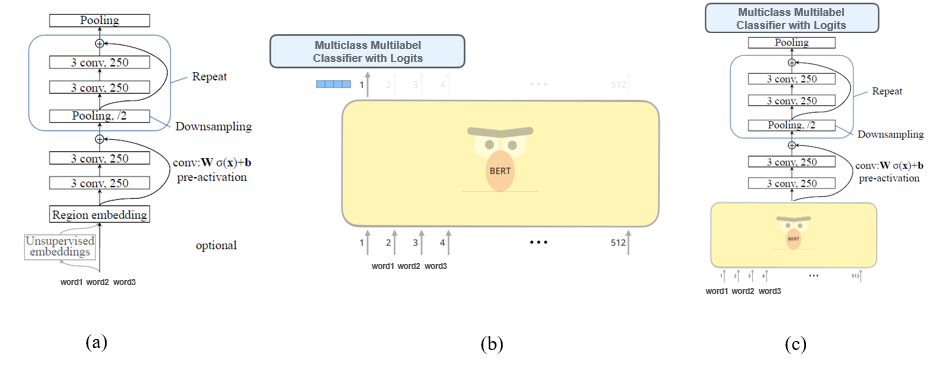
\includegraphics[scale=0.4]{images/bert_and_dpcnn.png}
    \caption{(a) Original DPCNN; (b) BERT with multilabel classifier; (c) BERT + DPCNN with multilabel classifier}
    \label{fig:bert_dpcnn_architecture}
\end{figure}

Our development was done with PyTorch and the Transformers\cite{huggingface_ref}, which allowed us to integrate with the weights of the pre-trained models. We re-implemented classes from the Transformers package to embed DPCNN into the fine-tuning process and also to change the loss computation, as explained in section \ref{metrics_section}. In this way, we trained BERT, XLNet and RoBERTa with and without the DPCNN. The training of the six models was done using NVIDIA Tesla K80 GPUs on Microsoft Azure and Google GCP for over 173 hours.

The data was divided into two sets, 80\% for training and 20\% for test. As some models took more than 30 hours to train with the full training set, we performed most of the hyperparameter tuning on a subset of the data (the articles for the year of 2004). This subset was also divided into two 80-20\% sets. We took this path due to hardware restrictions and assumed that the hyperparameters would to some degree generalize for the full dataset. In sum, the reported results relates to the performance of the models on the test sets, after training them on the full training sets with hyperparameters obtained in subset of the training set.


\section{METRICS} \label{metrics_section}

For the NYT multiclass multilabel classification problem we have to change the way the loss function is calculated by making use of a \textit{Binary Cross-Entropy with Logits} (\textit{torch.nn.BCEWithLogitsLoss}) loss function instead of vanilla cross-entropy loss. The binary cross-entropy loss allowed our model to assign independent probabilities to the labels by assessing each logit independently as opposed to SoftMax approach. Our custom accuracy implementation function considered a threshold of 0.5 (assignment of a label to an observation of the corresponding logit of the class is greater than 0.5).
We found that for a multi-label classification problem, the ROC-AUC curve and F1 score are more reliable metrics. We calculated ROC-AUC and F1 score for each label separately. We calculated the micro-averaging on top of individual labels’ roc-auc scores to report our results.

\section{RESULTS} \label{result_section}

The overhead of DPCNN on training was very small. The DPCNN increases the flexibility of the model with the cost of a higher number of parameters. Nonetheless, this extra-flexibility resulted in better performance since the losses during training time were lower. The table \ref{table:training_results} summarizes the training results. It is worth noting that during the comparison of XLNet and XLNet + DPCNN, we maintained XLNet with the same hyperparameters in both settings. The same idea applied to BERT and RoBERTa.

During the XLNet model training with the full training set, we faced convergence problems and the loss in each epoch was kept substantially high when compared with other models. This problem did not happened during the testing phase of the ensembles (with 5000 observations), but we decided to report the bad results anyway since we reached time constraints to keep retraining XLNet (each XLNet epoch took about 11hs to complete). 

\clearpage
\begin{table}
\centering
 \begin{tabular}{ | c | c | c | c |} 
 \hline
 Model & Epochs & Last Epoch Train Loss & Time per Epoch (h) \\
 \hline
 BERT & 5 & 0.0013094 & 5.63 \\
 \hline
 BERT + DPCNN & 5 & 0.0010743 & 5.56 \\
 \hline
 XLNet & 3 & 0.2961464 & 11.06 \\
 \hline
 XLNet + DPCNN & 3 & 0.0857150 & 11.83 \\
 \hline
 RoBERTa & 3 & 0.0078878 & 7.93 \\
 \hline 
 RoBERTa + DPCNN & 3 & 0.0014001 & 8.37 \\
 \hline
\end{tabular}
\caption{Training results}
\label{table:training_results}
\end{table}

After training the model we calculated the Precision, Recall, F1-Score and ROC-AUC score on the test set. The results are shown in the table \ref{table:test_metrics}.

\begin{table}
\centering
\begin{tabular}{lrrrr}
\toprule
           Model &  Precision &    Recall &  F1-Score &   ROC-AUC \\
\midrule
            Bert &   0.878209 &  0.863113 &  0.870178 &  0.874779 \\
    Bert + DPCNN &   0.881649 &  0.859173 &  0.869258 &  0.873668 \\
           XLNET &   0.102867 &  0.034944 &  0.052167 &  0.504241 \\
   XLNET + DPCNN &   0.885762 &  0.818550 &  0.844268 &  0.826432 \\
         RoBERTa &   0.899204 &  0.875554 &  0.883765 &  0.882264 \\
 RoBERTa + DPCNN &   0.904194 &  0.869321 &  0.882721 &  0.875583 \\
\bottomrule
\end{tabular}
\caption{Test metrics for BERT, XLNet and RoBERTa with and without DPCNN}
\label{table:test_metrics}
\end{table}

Adding DPCNN consistently increased the precision of the model. Except for XLNet, the recall decreased slightly with DPCNN. When the two metrics were combined to create the F1 score the scores stayed about the same for BERT and RoBERTa and improved for XLNet. For the ROC-AUC score the results were roughly the same for BERT, better for XLNet and slightly worse for RoBERTa. The precision, recall and F1 score for the different labels is shown table \ref{table:test_metrics}. For the precision, recall, F1 score, percentage of correctly identified labels see \ref{appendix_precision_recall_model}; for the confusion matrix see \ref{appendix_confusion_matrices}.

Section \ref{appendix_classification_examples} in the appendix contains examples of sentences that were correctly classified. 'Business', 'Spots' and 'Obituary' were the labels that the classifiers obtained higher precision. To some degree that's expected because those categories have 'almost unique' words that occur with high frequency such as 'NASDAQ', 'football' and 'passed away', respectively. The labels with the lowest precision were 'Front Page' and 'Education'. The 'Front Page' always belonged to at least one more category (such as 'Business', 'US' or 'World') making it hard for the classifier to identify it correctly. For 'Education' the number of samples was relatively small.

\section{CONCLUSION} \label{conclusion_section}

We achieved better results in most performance metrics by stacking and fine-tuning together DPCNN with XLNet, BERT or RoBERTa, than by fine-tuning plain vanilla XLNet, BERT or RoBERTa models alone. Our conclusion is that DPCNN continues to be a powerful classification tool, since better results came with little time overhead during training. We believe that we could have achieved even better results if we had at our disposal more hardware, so we could have tried more fine-tuning options. Another further step that we believe that could also have increased performance is the addition of an extractive or abstractive summarization layer to our ensemble, so that the length of the input tokens wouldn't need to be much more than our limited choice of 128, when compared to the typical 1024-length of the NYT corpus.     

\newpage
\begin{thebibliography}{1}
\bibitem{dpcnn_ref}
Johnson, Rie  and Zhang, Tong
\newblock Deep Pyramid Convolutional Neural Networks for Text Categorization
\newblock {\em https://www.aclweb.org/anthology/P17-1052}

\bibitem{xlnet_ref}
Zhilin Yang, Zihang Dai, Yiming Yang, Jaime Carbonell, Ruslan Salakhutdinov, Quoc V. Le. 
\newblock XLNet: Generalized Autoregressive Pretraining for Language Understanding. 
\newblock arXiv:1906.08237v1 [cs.CL] 19 Jun 2019

\bibitem{bert_ref}
Jacob Devlin, Ming-Wei Chang, Kenton Lee, and Kristina Toutanova. 
\newblock Bert: Pre-training of
deep bidirectional transformers for language understanding.
\newblock arXiv:1810.04805v2 [cs.CL] 24 May 2019

\bibitem{roberta_ref}
Yinhan Liu et.al. 
\newblock RoBERTa: A Robustly Optimized BERT Pretraining Approach 
\newblock arXiv:1907.11692v1 [cs.CL]

\bibitem{nyt_corpus_ref}
Sandhaus, Evan. 
\newblock The New York Times Annotated Corpus Overview

\bibitem{sentencepiece_ref}
Taku Kudo and John Richardson. 
\newblock Sentencepiece: A simple and language independent subword tokenizer and detokenizer forneural text processing. 
\newblock arXiv preprint arXiv:1808.06226, 2018

\bibitem{machine_translation_ref}
Rico  Sennrich,  Barry  Haddow  and  Alexandra  Birch.   
\newblock Neural  Machine  Translation  of  Rare  Words  with  Subword  Units.
\newblock arXiv:1508.07909v5 [cs.CL] 10 Jun 2016

\bibitem{deepcontextualized_word_ref}
Matthew E. Peters, Mark Neumann, Mohit Iyyer, Matt Gardner, Christopher Clark, Kenton Lee, Luke Zettlemoyer.  
\newblock Deepcontextualized word representations. 
\newblock arXiv:1802.05365v2 [cs.CL] 22 Mar 2018

\bibitem{improving_language_understanding_ref}
Alec  Radford,  Karthik  Narasimhan,  Tim  Salimans,  and  Ilya  Sutskever.  
\newblock Improving  language  understanding  with unsupervised learning. 
\newblock   2018.  Technical report, OpenAI.

\bibitem{huggingface_ref}
https://github.com/huggingface


\end{thebibliography}

\newpage
\section{APPENDIX}

\subsection{Full Examples} 

\textbf{Example 1: Long text with multiple labels} \label{appendix_example_1}
\newline
\newline
\textit{HEADLINE}
\newline
\newline
More than 40 prominent research universities have agreed not to accept direct Congressional grants for scientific facilities if the grants involve projects whose scientific merits have not been proved through competitive review.
\newline
\newline
\textit{NEWS ARTICLE}
\newline
\newline
More than 40 prominent research universities have agreed not to accept direct Congressional grants for scientific facilities if the grants involve projects whose scientific merits have not been proved through competitive review.

Because such grants bypass the normal review and are often awarded as a result of politicking by lobbyists hired by universities, they have been attacked as a potential danger to American research.

The universities involved make up most of the membership of the Association of American Universities, which was polled by mail over the past few weeks on the question of a moratorium on accepting such grants.

The vote approved a resolution that was drafted in response to a report last March by a special panel representing six higher education associations, including the A.A.U. The groups' take in many of the nation's most prestigious research universities, including Harvard, Yale, the Massachusetts Institute of Technology, and Columbia. A Growing Reliance

The issue centers on universities' growing reliance on special grants from Congress, earmarked for special purposes, as a source of Federal funds for building or renovating research facilities. The report that prompted the A.A.U.'s vote against such grants warned that university-based research would face "serious and lasting damage" if Congress continued the practice.

On the other hand, universities that have favored such grants maintain that they are merely righting an imbalance that has kept Federal money in the hands of prestigious schools in the Northeast and California.

They contend that in bypassing competitive scientific review procedures, Congress is rightly taking into account other considerations, such as economic development.

The Reagan Administration and numerous scientific agencies oppose earmarked grants, but opinion in Congress is divided. Congressional awards grew to $137 million in 1985 from $3 million in 1982, putting increased pressure on members of Congress to fight for special funds in their districts. Pressure on Congress Urged

The Association of American Universities was the first of the six academic organizations sponsoring the report on earmarked grants to act on it. The vote was 43 universities in favor of the moratorium, 10 opposing and 2 abstaining.

Robert M. Rosenzweig, president of the association, has told its members he does not think sanctions should be imposed on those who do not abide by the moratorium. He said the A.A.U. would urge the other organizations to join the moratorium and to push for Congressional passage of a system of financing or constructing scientific facilities.

In the interim, Mr. Rosenzweig added, the association will fight any effort to extend earmarking to cover funds for scientific projects but will not engage in "vain efforts" to oppose specific earmarked grants for research buildings, once they come up in Congress. A Defense by Columbia

Columbia University, which voted against the moratorium, regarded it as a potential affront to Congress, according to Gregory Fusco, vice president for governmental relations.

"Our concern was that the resolution as crafted would be interpreted in Congress as not giving sufficient recogition to the role of Congress in determining the uses of Federal funds," Mr. Fusco said. "We think Congress's consideration of economic development in addition to scientific merit is a valid one. It's valuable and appropriate." But he added that Columbia agreed with that portion of the A.A.U. resolution that called for seeking the creation of new Federal programs to help support university research facilities.

"We do need a big facilities program on the Federal level," he said. "Government should not pay for every facility in the country, but it should take a bigger responsibility than it has been. That's the main thing, and within the A.A.U. there's no dispute on that."
\newline
\newline
\textit{LABELS: Front\_Page, US, Education, Science, Technology}
\newline
\newline
\textbf{Example 2: Short text with a single label} \label{appendix_example_2}
\newline
\newline
\textit{NEWS ARTICLE}
\newline
\newline
To the Sports Editor:
In his analysis of this season's most valuable player candidates ("This Season's Most Valuable Player, Pro and Con," The Times, Sept. 24), Murray Chass is quite right to point out that Albert Belle's contribution to the Indians' success is diminished somewhat by the presence in the Cleveland lineup of several other productive hitters. But to imply that the Seattle Mariners' Edgar Martinez's claim on the award is thereby better justified is to ignore that Martinez's batting mates are likewise formidable. Tino Martinez (29 home runs, 102 r.b.i.), Jay Buhner (35 homers, 112 r.b.i.) and Mike Blowers (22 homers, 93 r.b.i.) are hardly chopped liver (or should I say, smoked salmon?). JONATHAN B. HELD  Brooklyn
\newline
\newline
\textit{LABELS: Sports}

\subsection{Classification Examples} \label{appendix_classification_examples}
\textbf{Examples of correctly classified sentences:}
\newline
\newline
\textbf{Sports:}
\newline
\newline
“The American Football Conference hasn't seen a team like these new Steelers since the old Steelers. But don't say it yet. Don't say "Super Bowl" even after they whipped the Browns, 29-9, on Saturday to move within a game of The Game. …”

“The transformation of the Jets in Rich Kotite's rookie season as their coach was nearly completed today, wrapping up as wild a weekend as the team has ever experienced.When it was over, they had traded still another starter, acquired one from the Giants, of all people, and drafted at least two players who are virtually certain to become starters. …”
\newline
\newline
\textbf{Business:}
\newline
\newline
“All three major stock market indexes fell for the third consecutive week as the prospect of a possible war with Iraq weighed on investors. A rally on Friday could not counter two weeks of deep losses. For January as a whole, the Dow fell 3.5 percent, the Nasdaq declined 1.1 percent …”

“Reflecting a slowing economy, inflation at the producer level disappeared again in May, as price declines for food and some energy products offset increases for other types of finished goods, Government figures showed today. Price pressures also eased at earlier stages of the production process, with the Producer Price Index for such intermediate components as bolts of cloth posting its smallest rise in a year. …”
\newline
\newline
\textbf{Examples of incorrectly classified sentences:}
\newline
\newline
\textit{Labeled “World” and “Front Page”, model predicted “World” and “Washington”:}
\newline
\newline
“Secretary of State Warren Christopher, worried that his efforts to repair relations with Beijing could be threatened, has demanded an investigation into why the Pentagon sent two officers to watch military exercises from the Chinese coast …”
\newline
\newline
\textit{Labeled “Technology”, model predicted “Sports” and “Business”:}
\newline

'SHIGERU MIYAMOTO can hardly walk through the streets of this city unnoticed. Entering a restaurant here last month with a group of other executives, he was immediately recognized by a waitress and asked for his autograph, one of 50 he would give that day. Some of those autographs were even given to employees at the United States offices of Nintendo in Redmond, Wash., where he had visited earlier in the day. Mr. Miyamoto, 46, remains surprised by his American celebrity. Back home at Nintendo\'s headquarters in Kyoto, Japan, he enjoys greater anonymity. "They do not ask me for my autograph," he says. Are you over 40 and unfamiliar with Mr. Miyamoto? Ask your children. Officially, Mr. Miyamoto is general manager of entertainment analysis and development at the Nintendo Company, the \$4.5 billion Japanese giant. Unofficially, to most video game software developers and aficionados, he is a deity."He's the god of gaming," said Jennifer Pahlka, director of the Game Developers Conference, an industry trade show, which gave Mr. Miyamoto its first lifetime achievement award in March, the occasion of his visit to San Jose.

\subsection{Distribution of Tokens}

\begin{figure}[!htb]
    \centering
    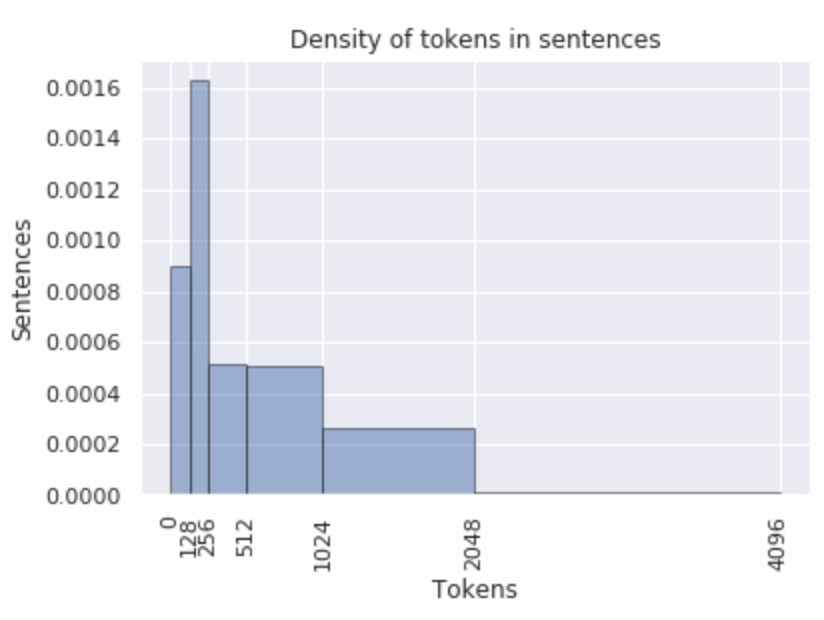
\includegraphics[scale=0.6]{images/density_tokens.png}
    \caption{Distribution of number of tokens in texts of the dataset. This plot was built using SetencePiece.}
    \label{fig:density_tokens}
\end{figure}

\subsection{Results} \label{apendix_results}

\subsubsection{Precision, Recall and F1 scores by Labels}

\begin{figure}[!htb]
    \centering
    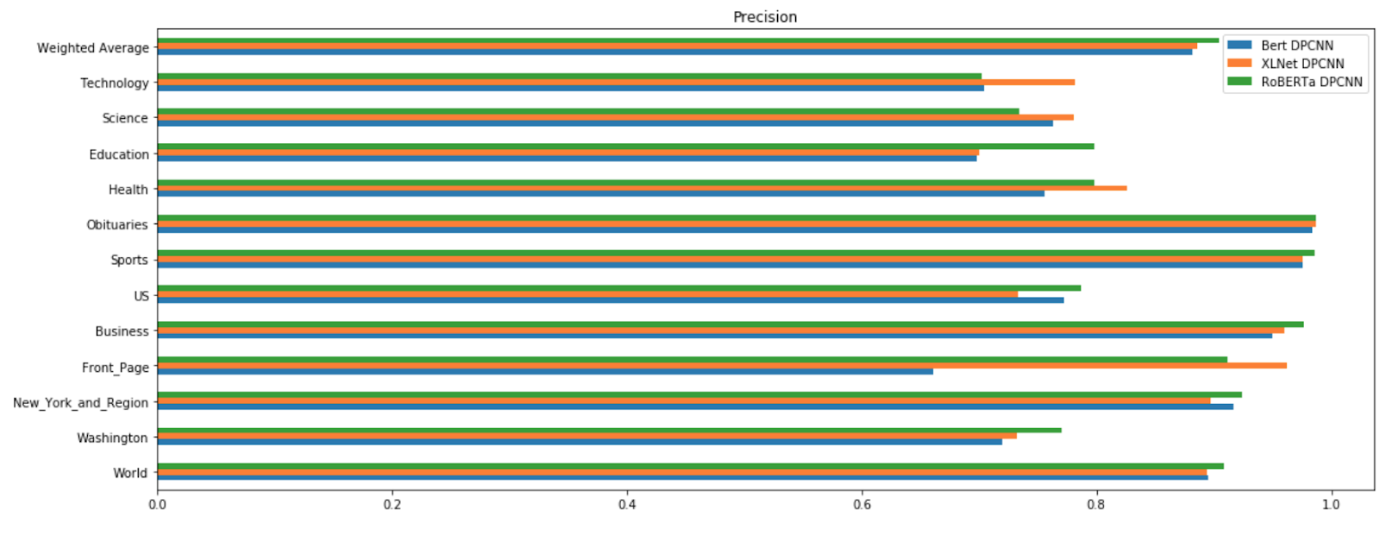
\includegraphics[scale=0.6]{images/precision_labels_all_models.png}
    \caption{Label precision for BERT, XLNet and RoBERTa with DPCNN}
    \label{fig:precision_labels_all_models}
\end{figure}

\begin{figure}[!htb]
    \centering
    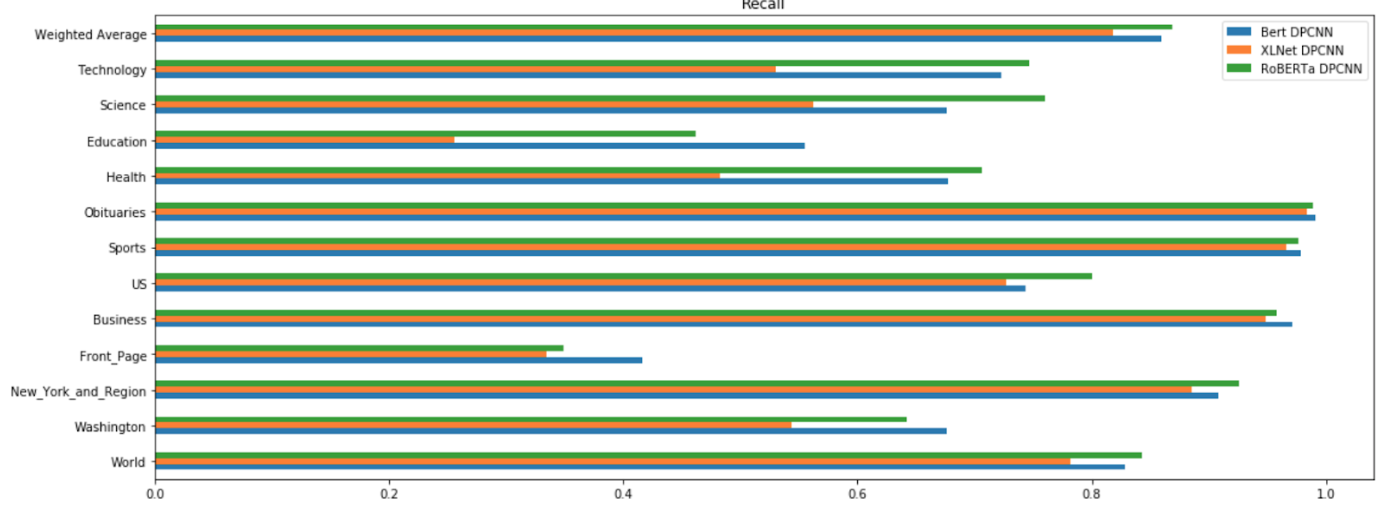
\includegraphics[scale=0.6]{images/recall_labels_all_models.png}
    \caption{Label recall for BERT, XLNet and RoBERTa with DPCNN}
    \label{fig:recall_labels_all_models}
\end{figure}

\begin{figure}[!htb]
    \centering
    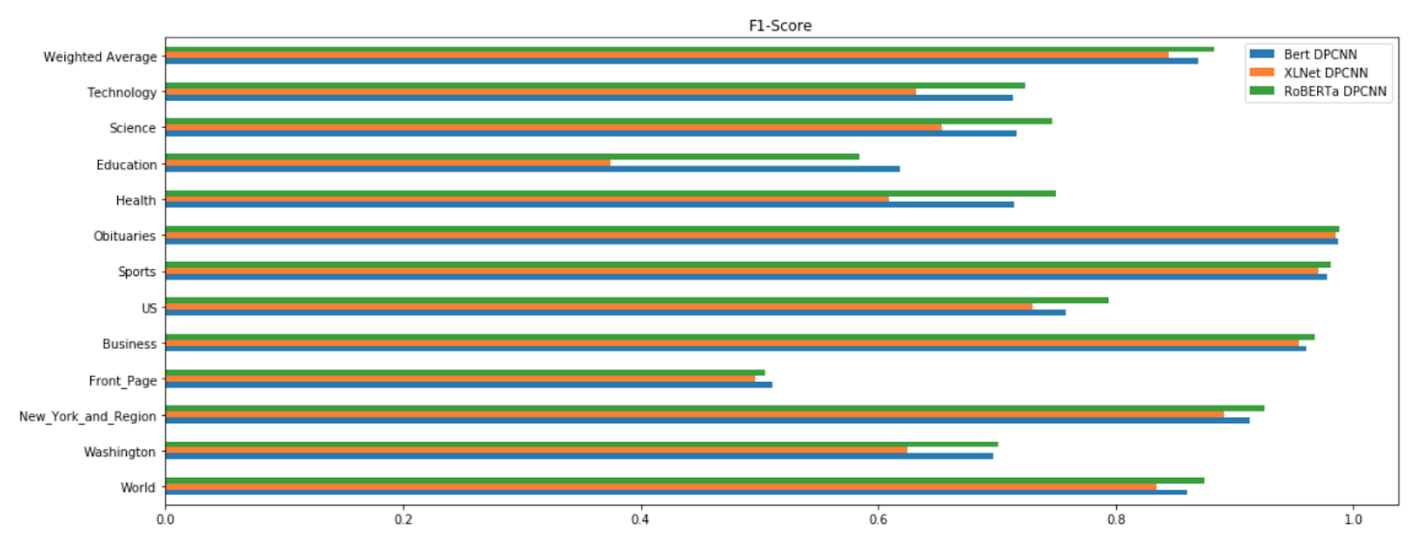
\includegraphics[scale=0.6]{images/f1_labels_all_models.png}
    \caption{F1 score for BERT, XLNet and RoBERTa with DPCNN}
    \label{fig:f1_labels_all_models}
\end{figure}

\clearpage
\newpage
\subsubsection{Precision and Recall by Model} \label{appendix_precision_recall_model}

\begin{figure}[!htb]
    \centering
    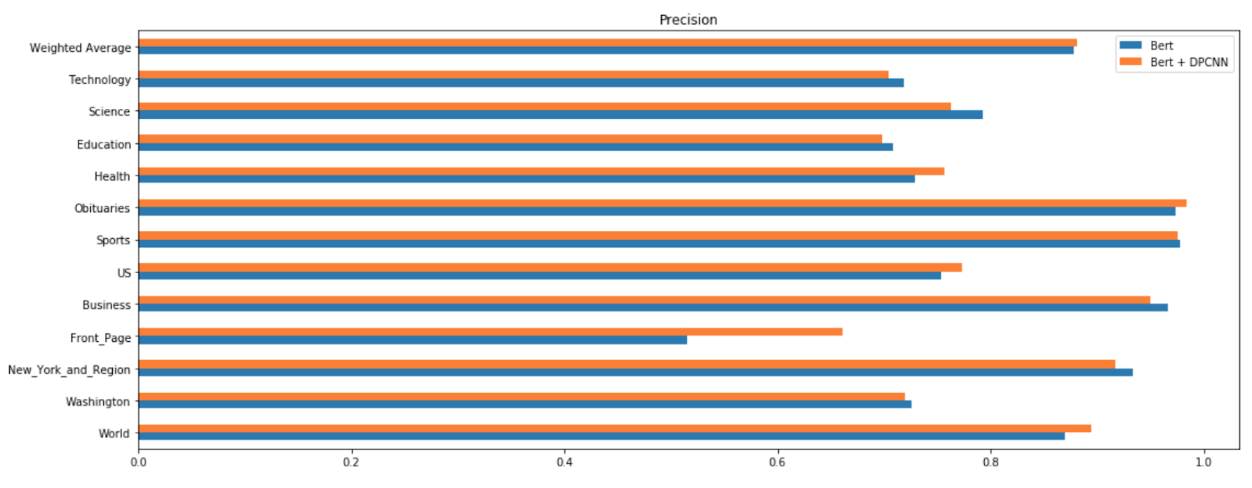
\includegraphics[scale=0.6]{images/precision_bert.png}
    \caption{Precision for BERT and BERT + DPCNN}
    \label{fig:precision_bert}
\end{figure}

\begin{figure}[!htb]
    \centering
    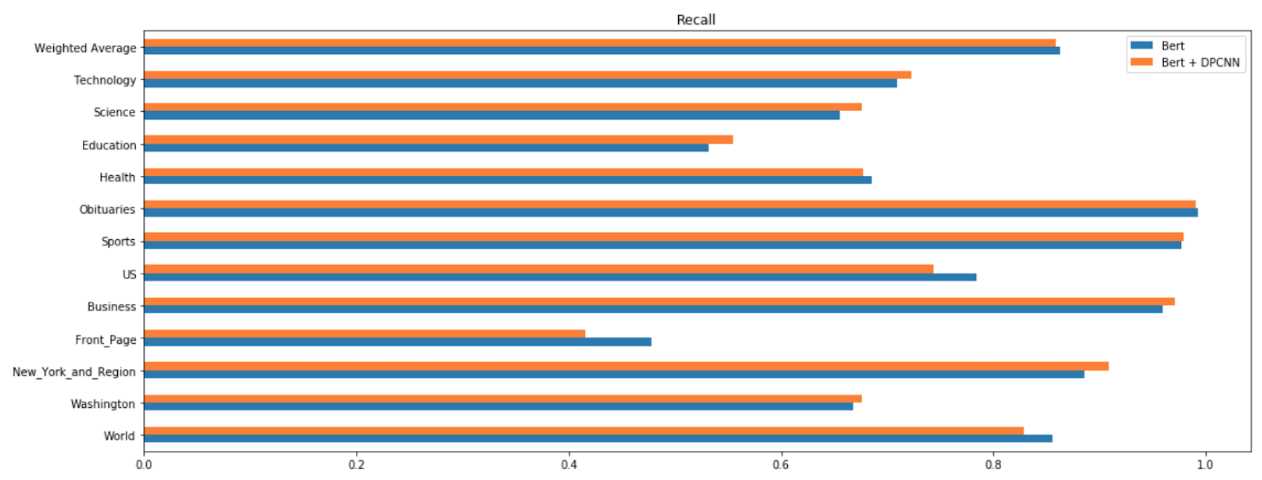
\includegraphics[scale=0.6]{images/recall_bert.png}
    \caption{Recall for BERT and BERT + DPCNN}
    \label{fig:recall_bert}
\end{figure}

\begin{figure}[!htb]
    \centering
    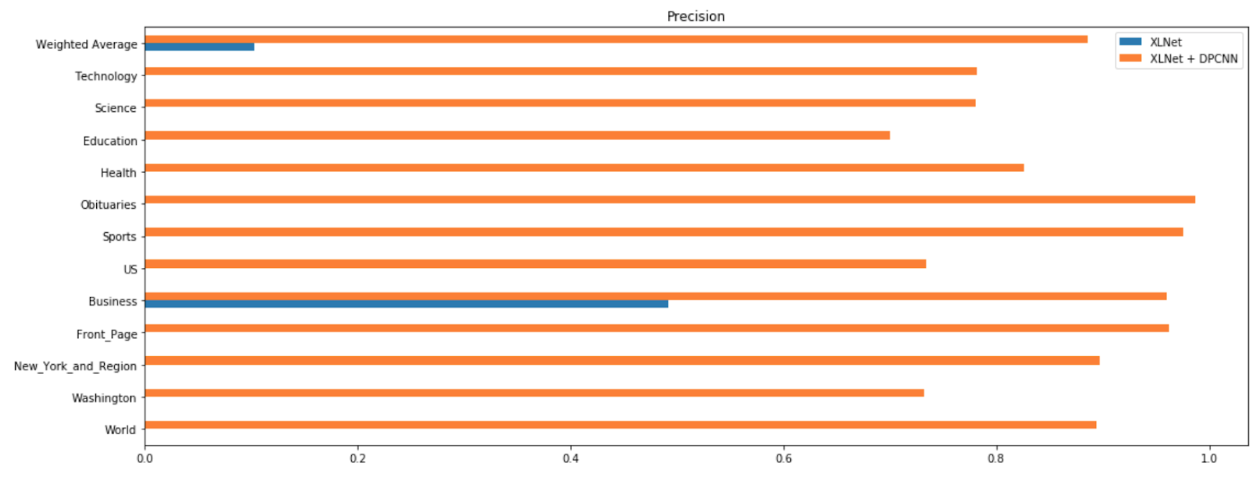
\includegraphics[scale=0.6]{images/precision_xlnet.png}
    \caption{Precision for XLNet and XLNet + DPCNN}
    \label{fig:precision_xlnet}
\end{figure}

\begin{figure}
    \centering
    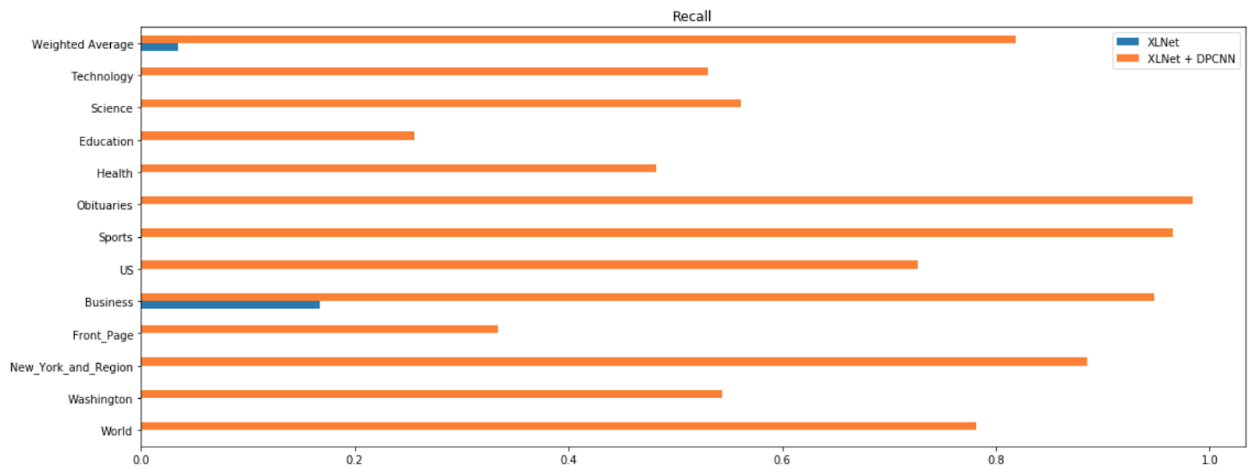
\includegraphics[scale=0.6]{images/recall_xlnet.png}
    \caption{Recall for XLNet and XLNet + DPCNN}
    \label{fig:recall_xlnet}
\end{figure}

\begin{figure}
    \centering
    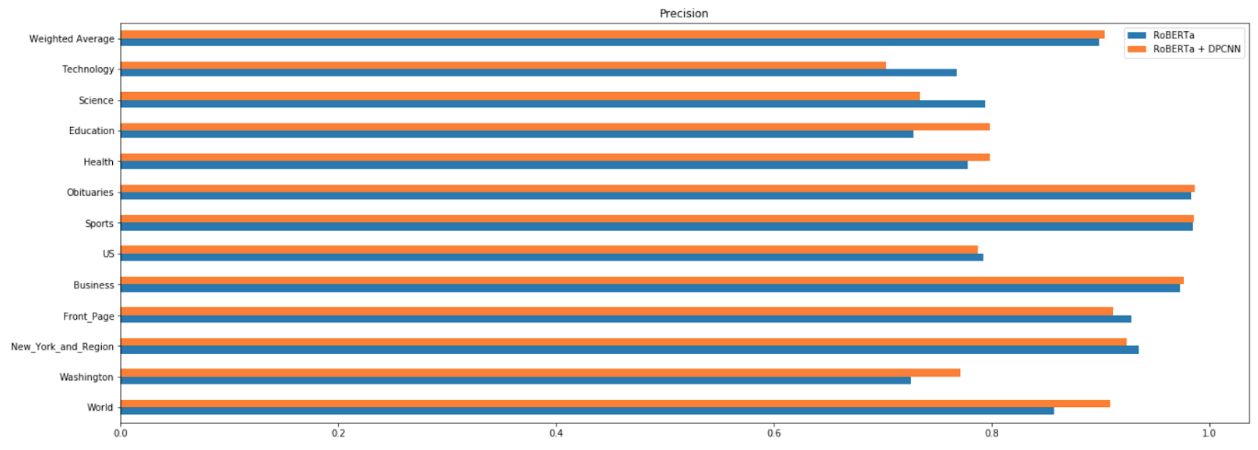
\includegraphics[scale=0.6]{images/precision_roberta.png}
    \caption{Precision for RoBERTa and RoBERTa + DPCNN}
    \label{fig:precision_roberta}
\end{figure}

\begin{figure}
    \centering
    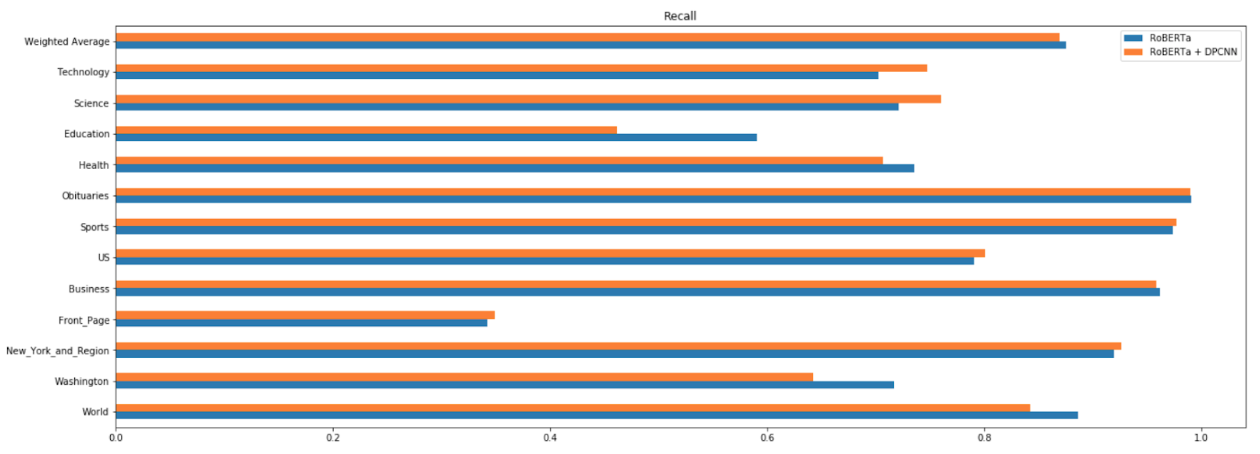
\includegraphics[scale=0.6]{images/recall_roberta.png}
    \caption{Recall for RoBERTa and RoBERTa + DPCNN}
    \label{fig:recall_roberta}
\end{figure}

\clearpage
\subsubsection{Confusion Matrices} \label{appendix_confusion_matrices}

Confusion matrices for articles with a single label for all the models.

\begin{figure}[!htb]
    \centering
    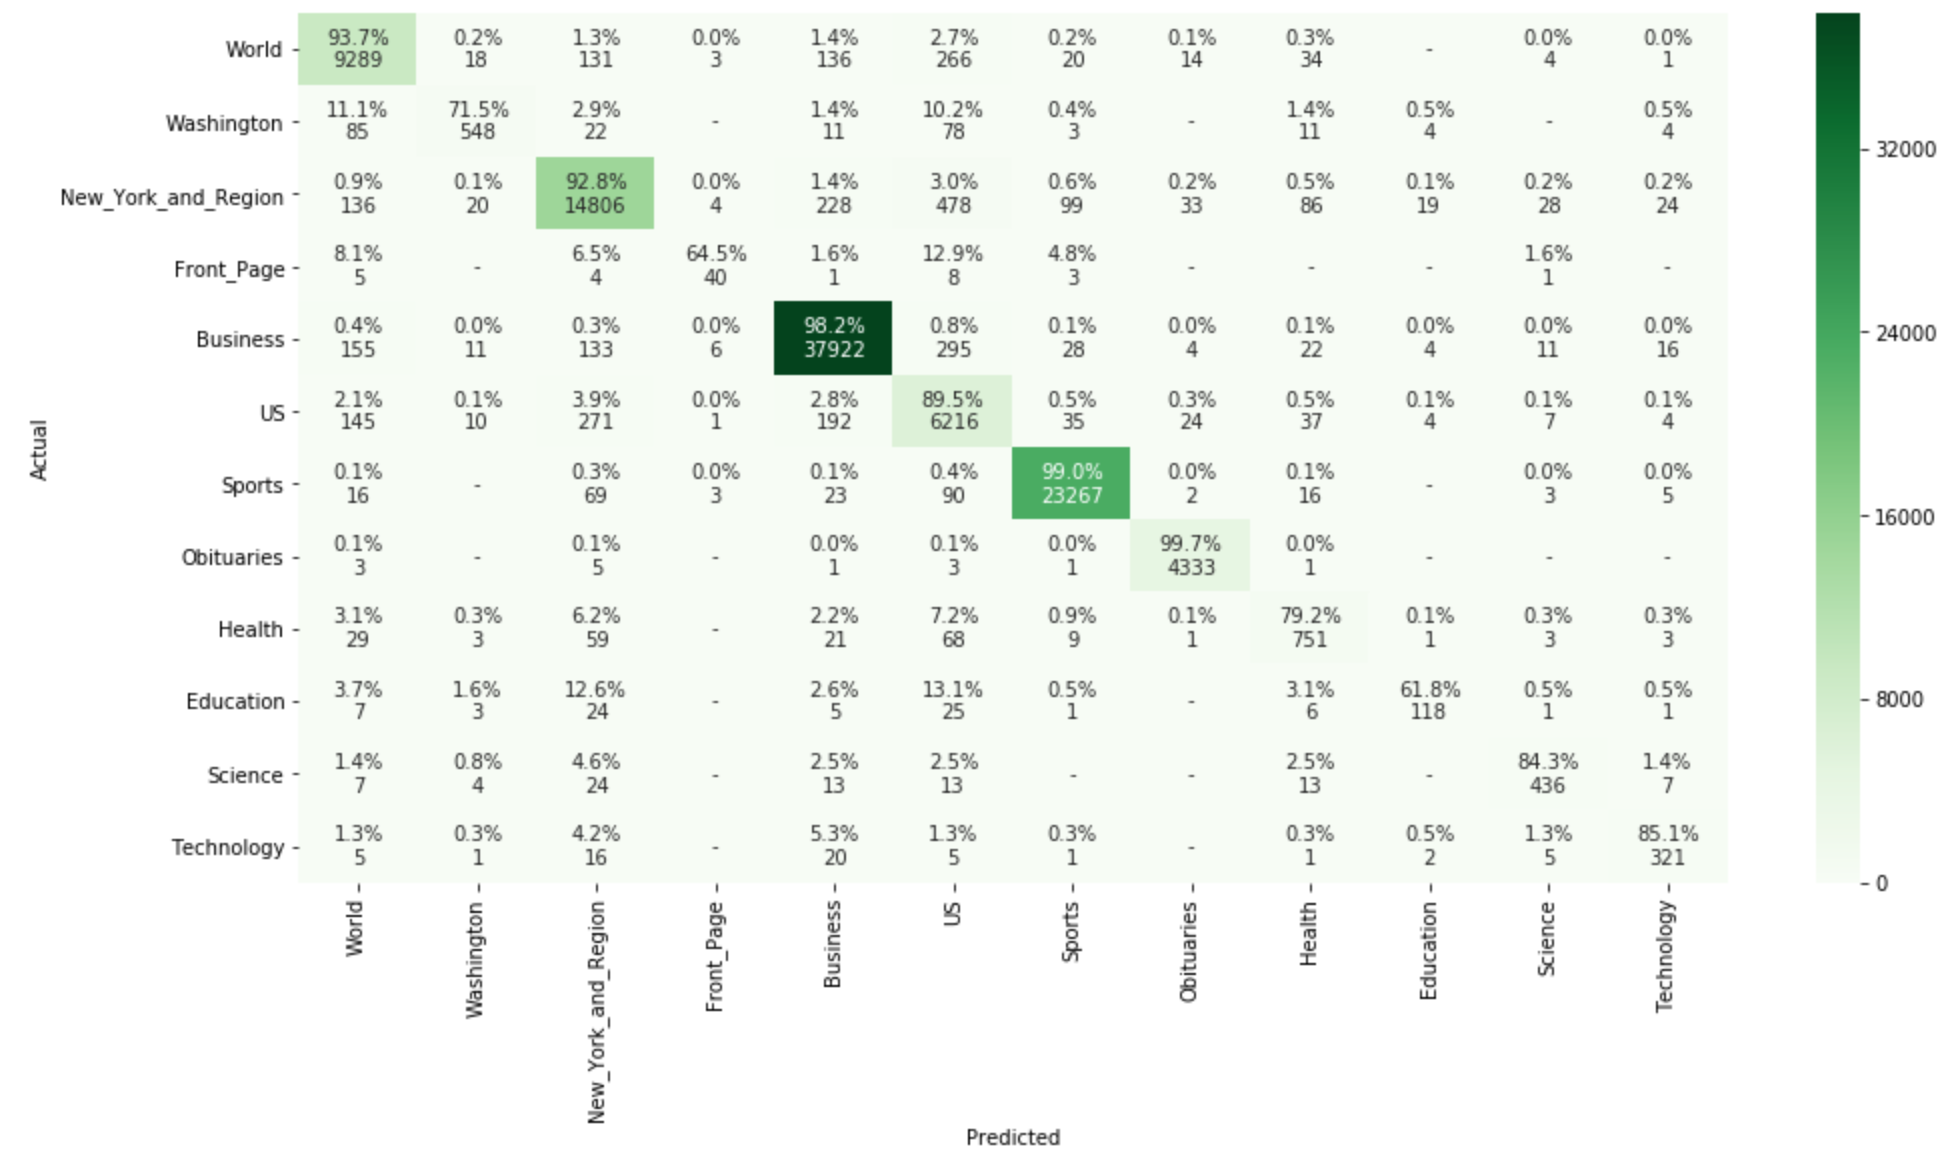
\includegraphics[scale=0.4]{images/confusion_bert.png}
    \caption{Confusion Matrix for single label articles for BERT}
    \label{fig:confusion_bert}
\end{figure}

\begin{figure}[!htb]
    \centering
    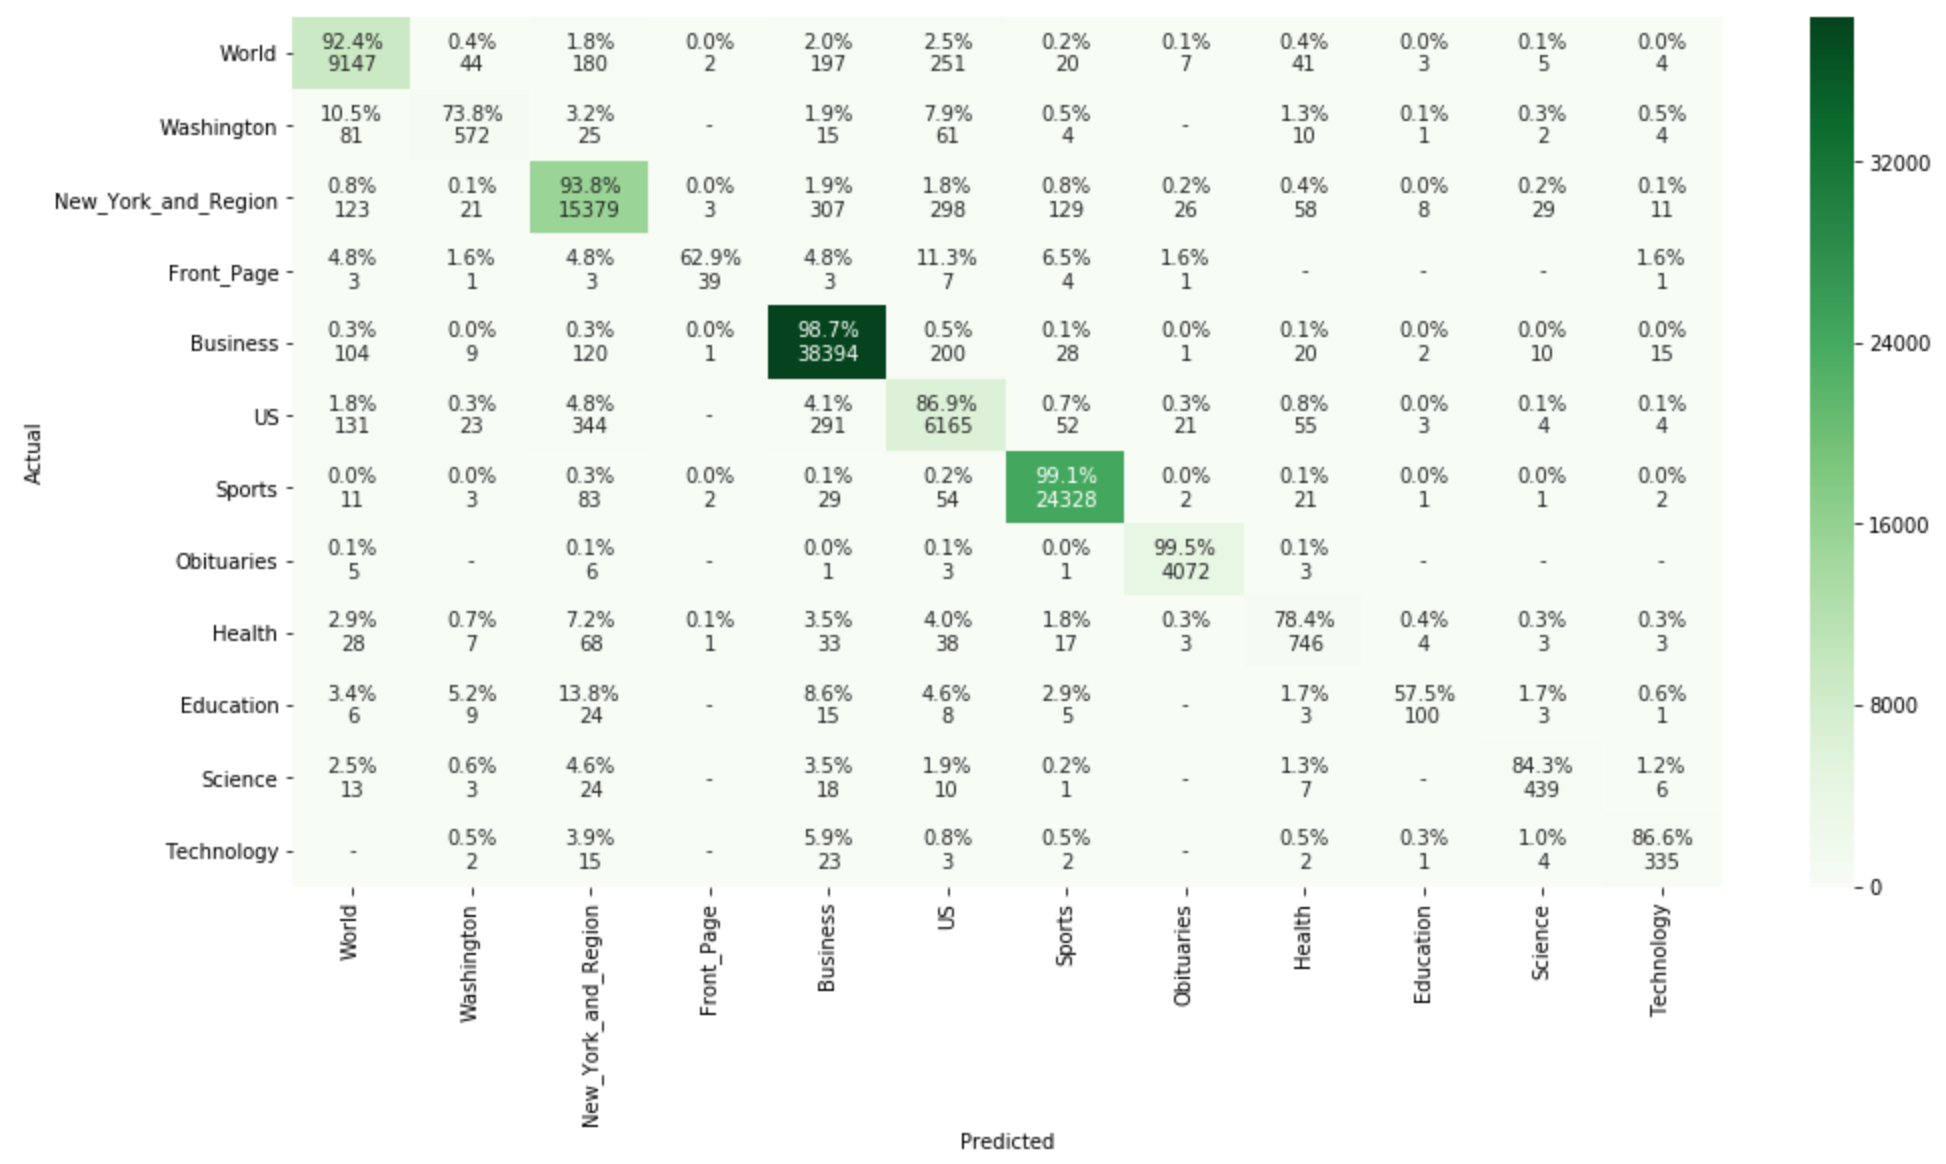
\includegraphics[scale=0.4]{images/confusion_bert_dpcnn.png}
    \caption{Confusion Matrix for single label articles for BERT + DPCNN}
    \label{fig:confusion_bert_dpcnn}
\end{figure}

\begin{figure}[!htb]
    \centering
    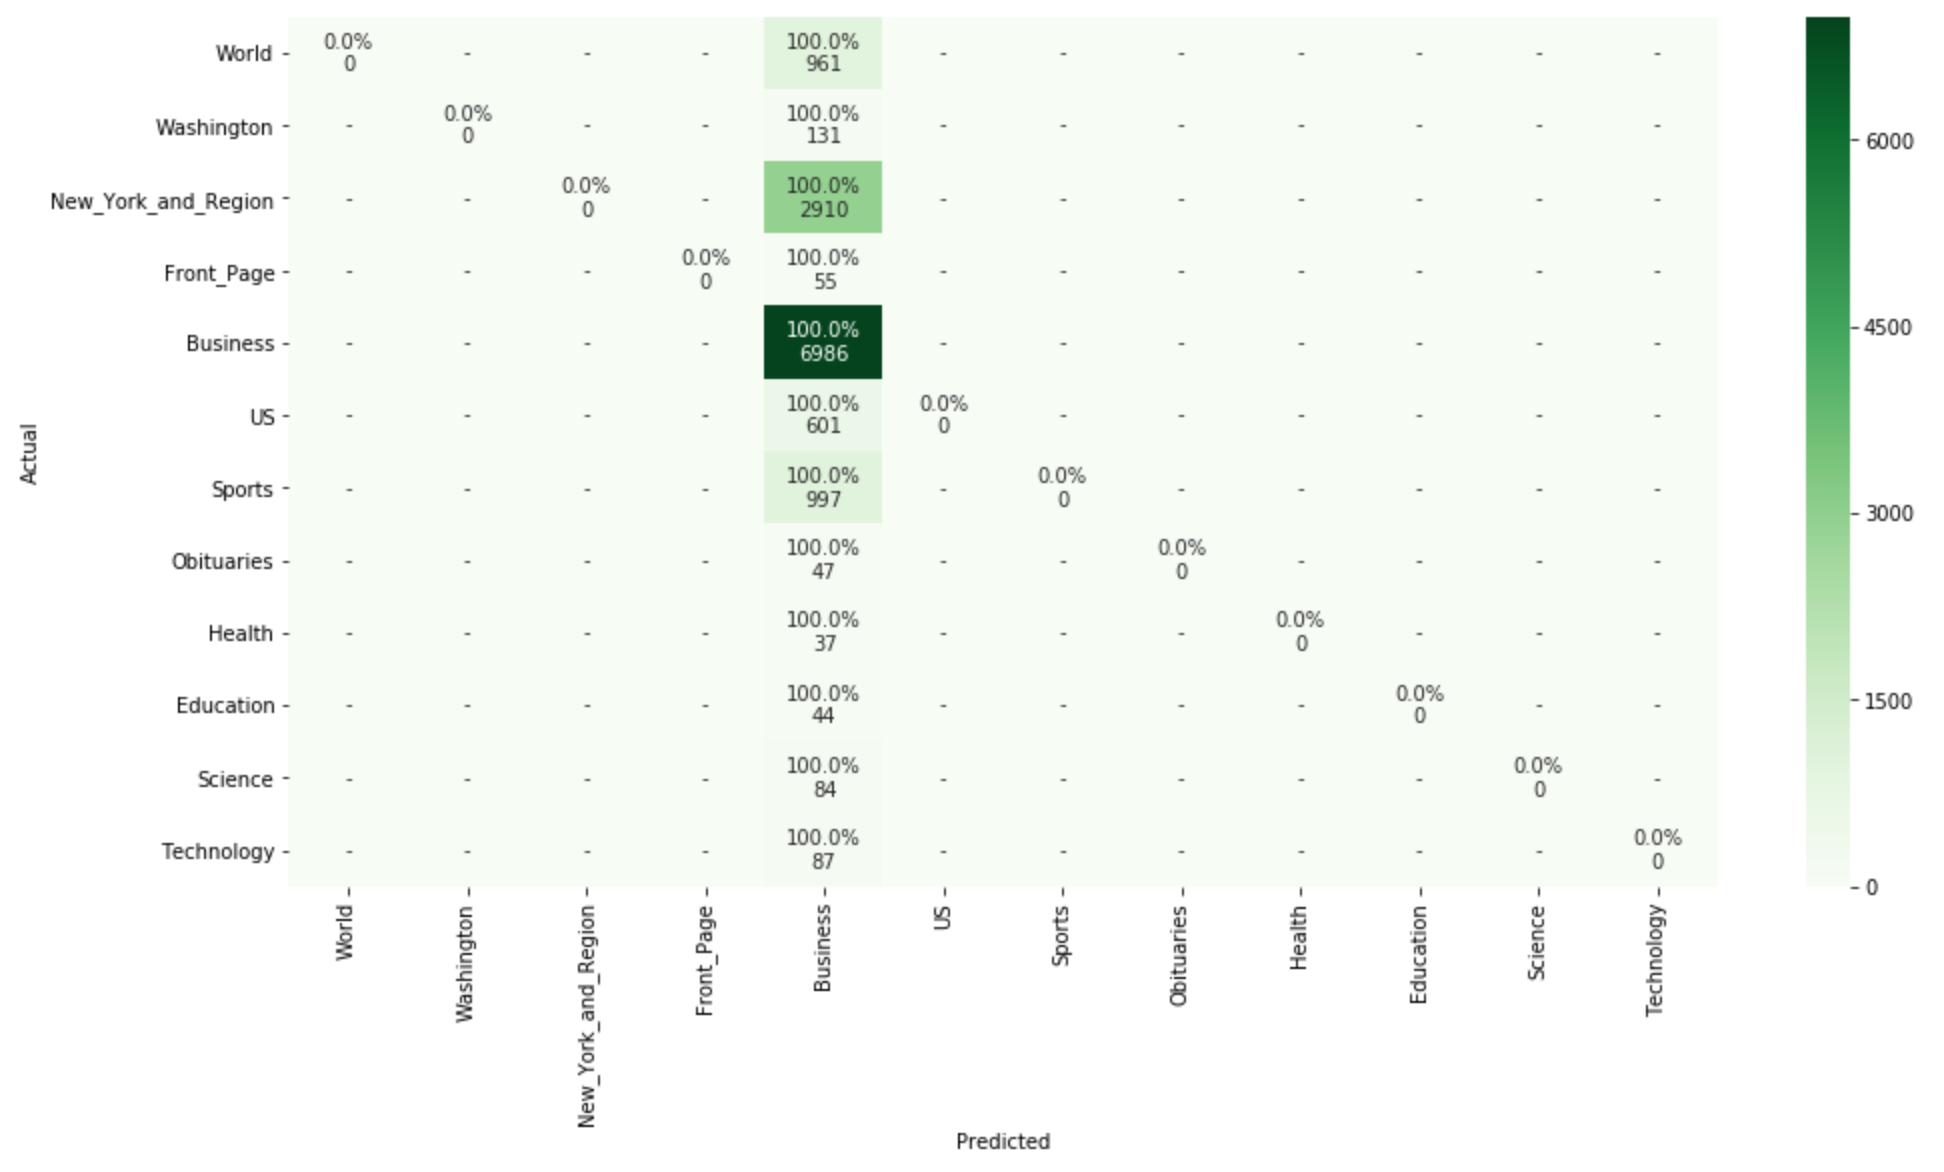
\includegraphics[scale=0.4]{images/confusion_xlnet.png}
    \caption{Confusion Matrix for single label articles for XLNet}
    \label{fig:confusion_xlnet}
\end{figure}

\begin{figure}[!htb]
    \centering
    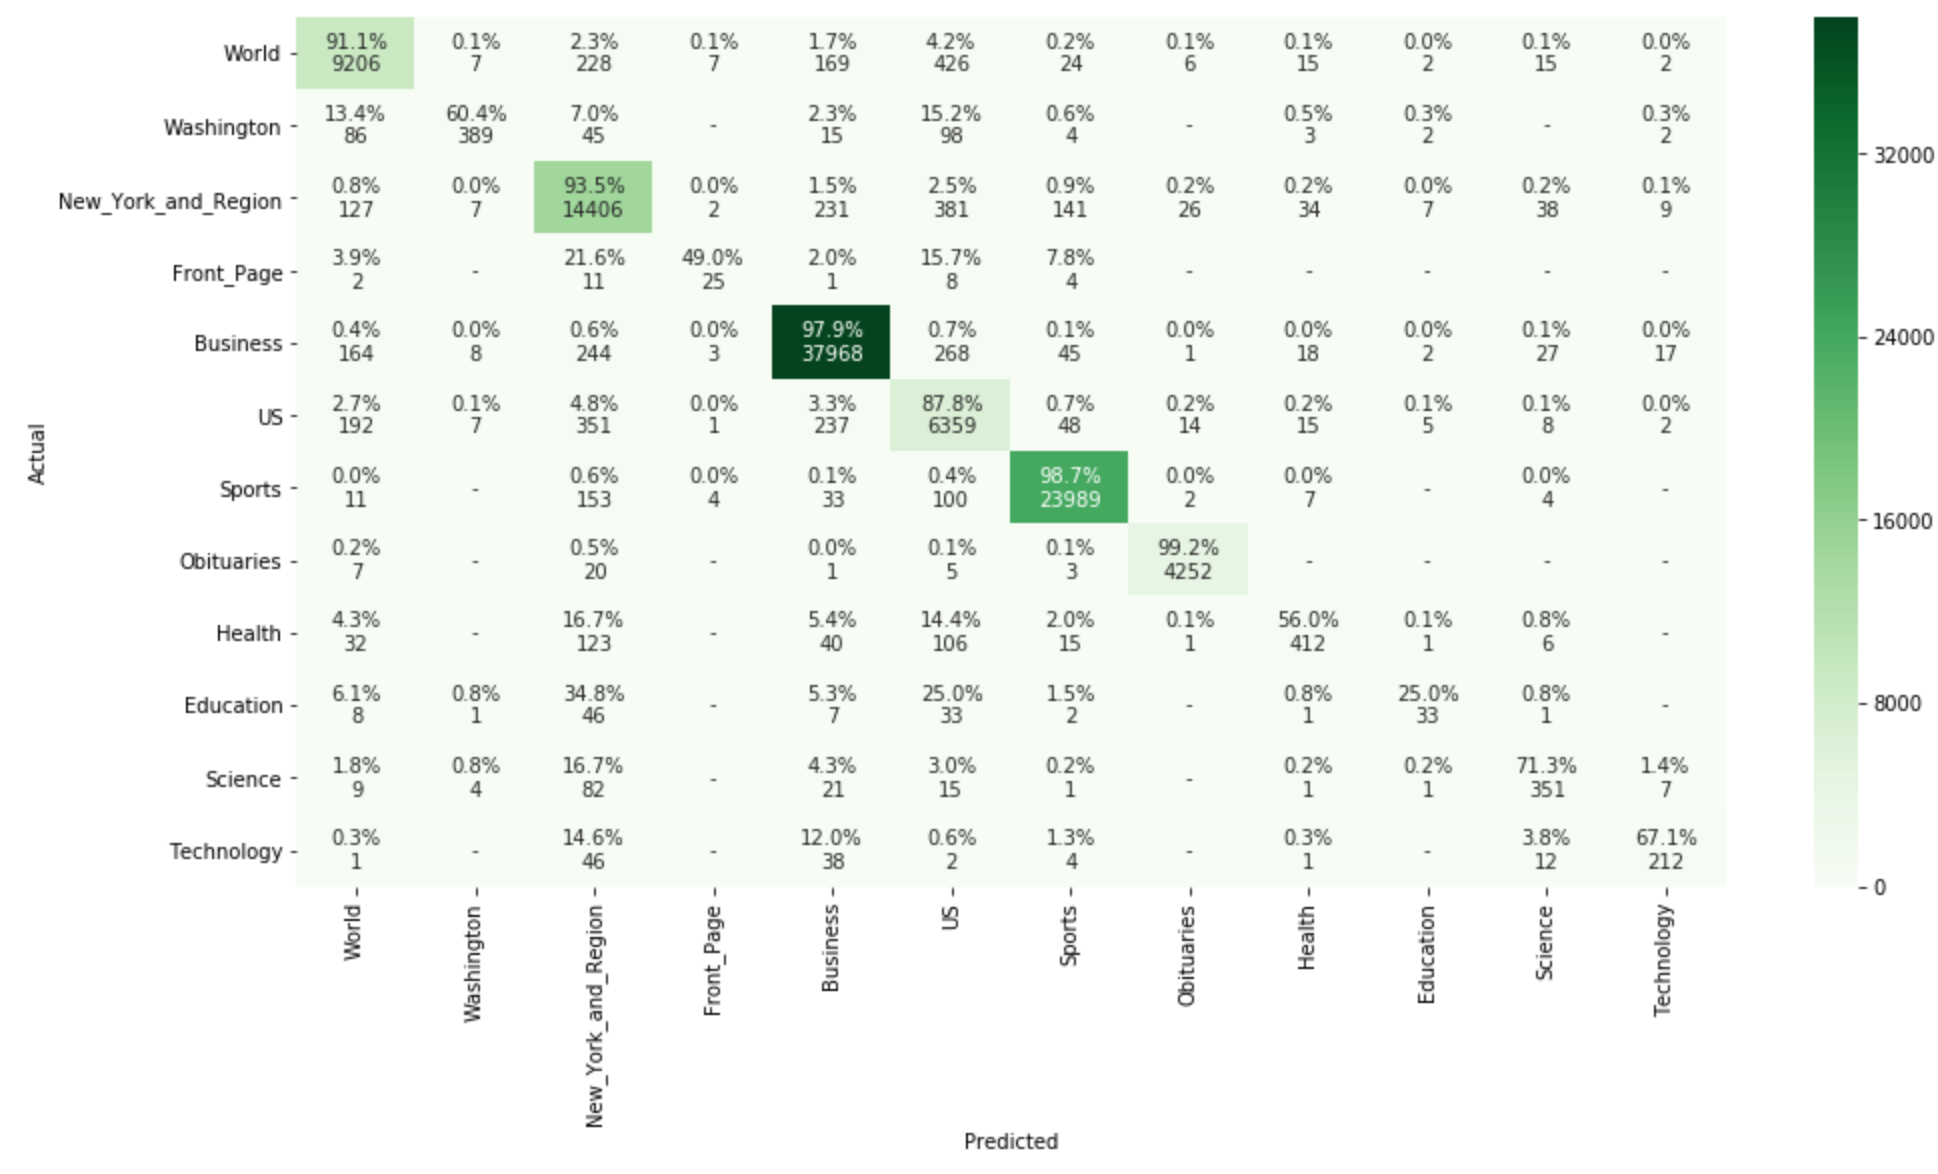
\includegraphics[scale=0.4]{images/confusion_xlnet_dpcnn.png}
    \caption{Confusion Matrix for single label articles for XLNet + DPCNN}
    \label{fig:confusion_bert_xlnet}
\end{figure}

\begin{figure}[!htb]
    \centering
    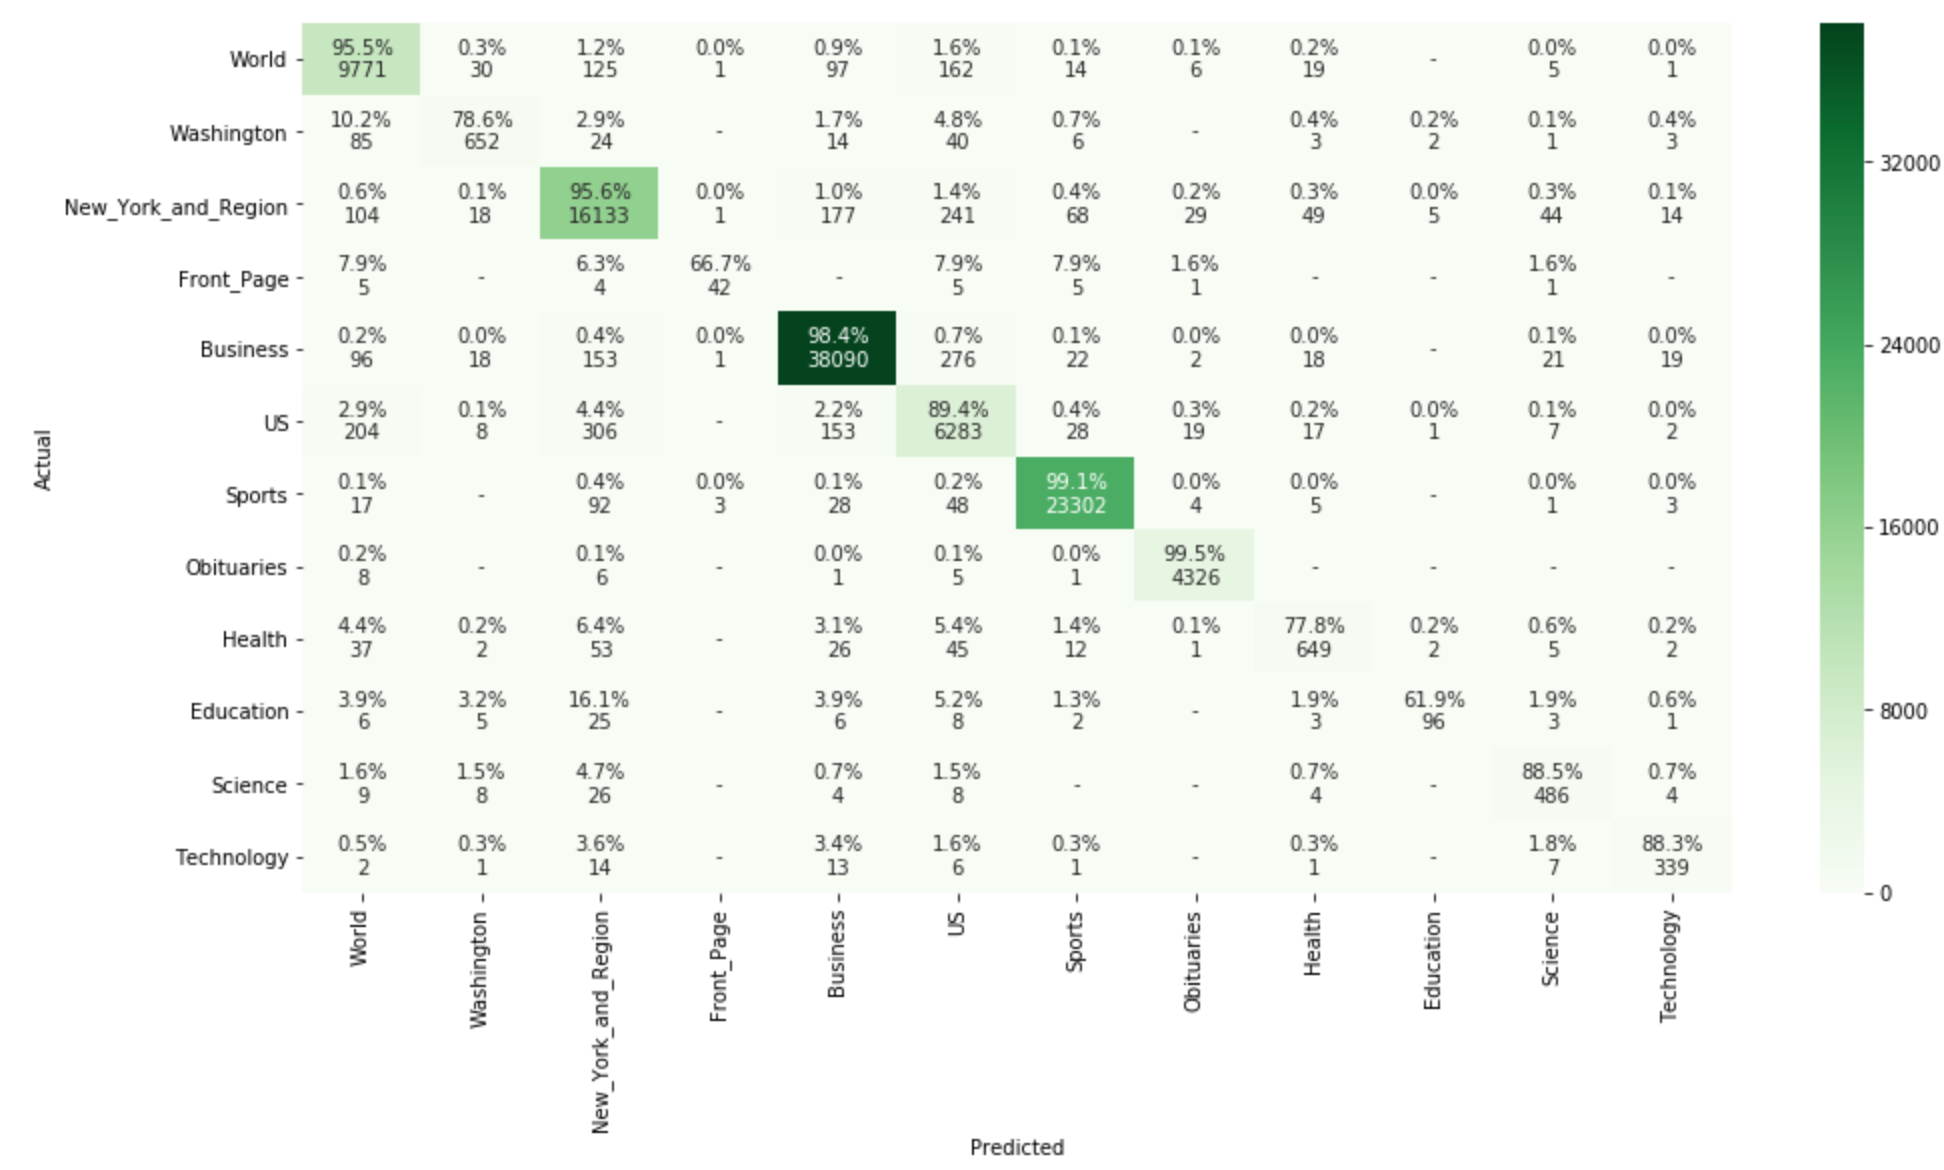
\includegraphics[scale=0.4]{images/confusion_roberta.png}
    \caption{Confusion Matrix for single label articles for RoBERTa}
    \label{fig:confusion_roberta}
\end{figure}

\begin{figure}[!htb]
    \centering
    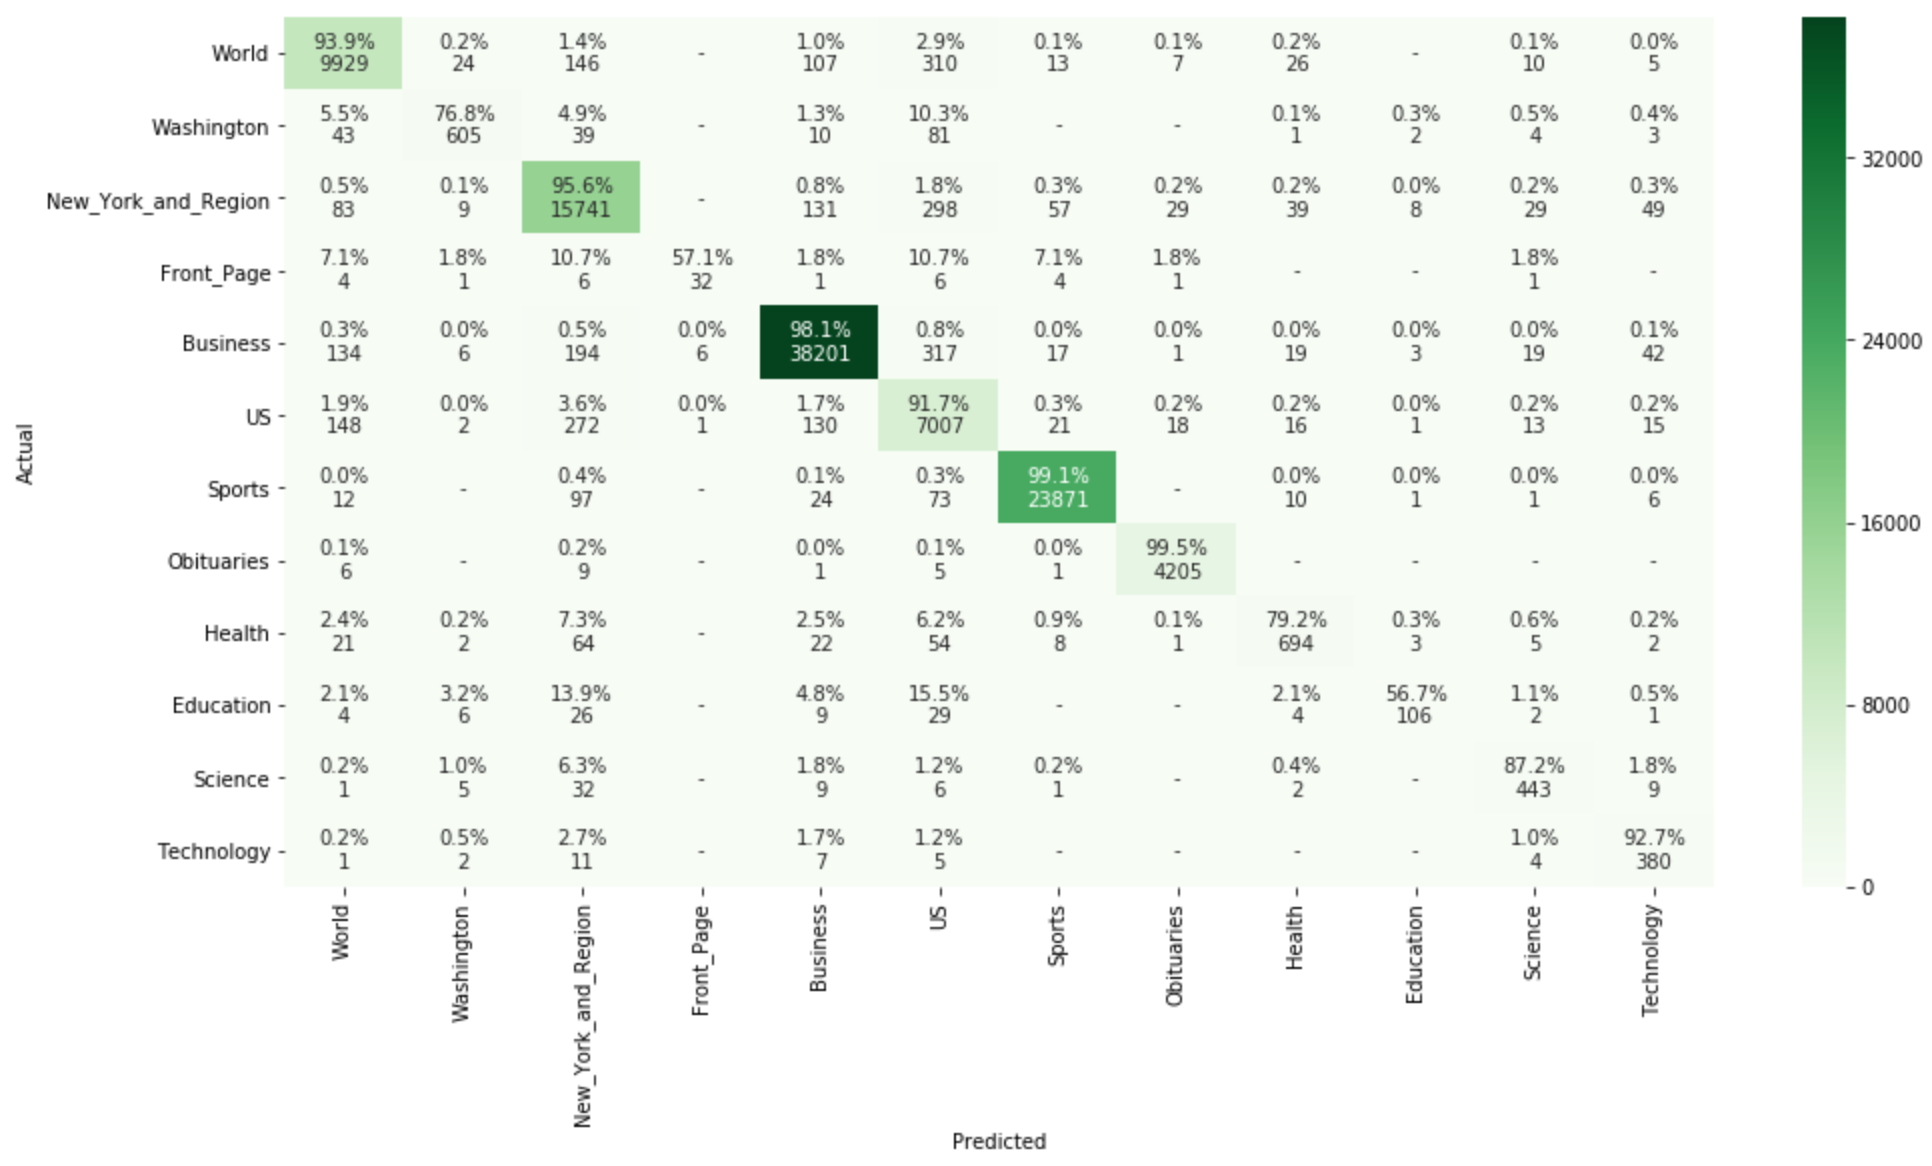
\includegraphics[scale=0.4]{images/confusion_roberta_dpcnn.png}
    \caption{Confusion Matrix for single label articles for RoBERTa + DPCNN}
    \label{fig:confusion_roberta_dpcnn}
\end{figure}


\end{document}